\chapter{Aktueller Stand der Forschung und Praxis (generell auch wiedergeben von aktuell existierenden Lösungsmustern)}

\section{Ressourcenverbrauch bei KI-Modellen}
\subsection{Ressourcenverbrauch bei KI-Modellen}
\subsubsection{Nachhaltigkeit}
\subsubsection{Stromverbrauch}
\subsubsection{Rechenleistung begrenzt, KI-Modelle wachsen schneller als verfügbare Leistung}

\section{Deep Neural Network - Boltzmann Maschinen (Erstmal DNN erklären generell)}
\subsection{Konzept und Anwendung des Modells }

A \ac{BM} is a symmetrical energy-based network consisting of neurons.\footcite[Vgl.][260]{amariInformationGeometryBoltzmann1992}
The neurons of the network can be split into two functional groups, a set of visible neurons and a set of hidden neurons.\footcite[Vgl.][154]{ackleyLearningAlgorithmBoltzmann1985}
Therefore, the \ac{BM} is a two-layer model and has a visible layer (``v'') and a hidden layer (``h'').\footcite[Vgl.][448]{salakhutdinovDeepBoltzmannMachines2009}
The visible layer is the interface between the network and the environment. It receives data inputs during training and sets the state of a neuron to either {0; 1} which represents activated or not activated.
On the other hand, the hidden units are not connected to the environment and can be used to “explain” underlying constraints in the ensemble of input vectors and they cannot be represented by pairwise constraints.\footcite[Vgl.][154]{ackleyLearningAlgorithmBoltzmann1985}
The connection between the individual neurons is referred to as bidirectional, as each neuron communicates with each other in both directions.\footcite[Vgl.][149]{ackleyLearningAlgorithmBoltzmann1985}
In the following visualization 1, a general \ac{BM} is depicted, where the upper layer embodies a vector of stochastic binary 'hidden' features, while the lower layer embodies a vector of stochastic binary 'visible' variables.\footcite[Vgl.][449]{salakhutdinovDeepBoltzmannMachines2009}

\begin{figure}[H]
    \centering
    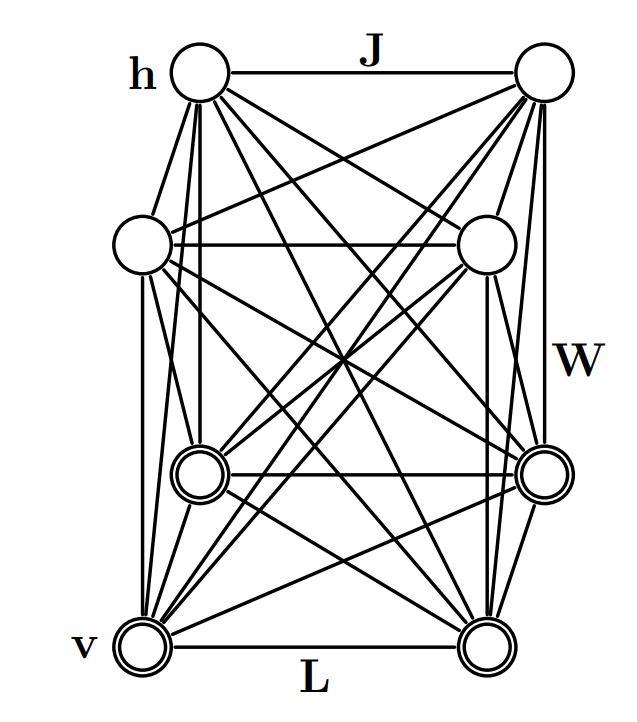
\includegraphics[width=0.25\linewidth]{graphics/General_BM.png}
    \caption{Visualization of a general \ac{BM}}
\end{figure}

It contains a set of visible units \( v \in \{0, 1\}^D \), and a set of hidden units \( h \in \{0, 1\}^P \) (see Fig. 1). The energy of the state \( \{v, h\} \) is defined as:

\begin{equation}
E(v, h; \theta) = -\frac{1}{2} v^T L v - \frac{1}{2} h^T J h - v^T W h
\end{equation}

where \( \theta = \{W, L, J\} \) are the model parameters.\footcite[448][Vgl.]{salakhutdinovDeepBoltzmannMachines2009}
\( W, L, J \) represent visible-to-hidden, visible-to-visible and hidden-to-hidden weights.
 

The network can update the weights ``W'' that exist between the neurons through specific training rules based on the observations that served as input.\footcite[Vgl.][1-2]{barraEquivalenceHopfieldNetworks2012}

As early as 1985, one of the founding fathers of artificial intelligence, ``Geoffrey Hinton'', was aware that an \ac{BM} is able to learn its underlying features by looking at data from a domain and developing a generative internal model.\footcite[Vgl.][148]{ackleyLearningAlgorithmBoltzmann1985}
In the next step, it is possible to generate examples with the same probability distribution as the examples shown.


\subsection{Energiefunktion}
\subsection{Training von BMs}





If the diagonal elements \( L \) and \( J \) of the general \ac{BM} introduced earlier, are set to 0 the known model of a \ac{RBM} establishes shown in fig.2.\footcite[Vgl.][449]{salakhutdinovDeepBoltzmannMachines2009}

\begin{figure}[H]
    \centering
    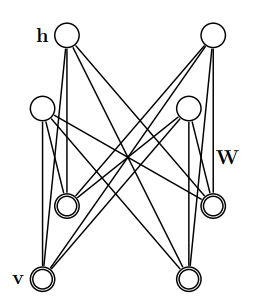
\includegraphics[width=0.25\linewidth]{graphics/RBM_Modell.png}
    \caption{Visualization of a \ac{RBM}}
\end{figure}
As a result no more visible-to-visible and hidden-to-hidden connections can be found in the network.
The configuration of the visible and hidden units \( (v, h) \) has an energy (Hopfield, 1982) given by:
\begin{equation}
E(v, h) = - \sum_{i \in \text{visible}} a_i v_i - \sum_{j \in \text{hidden}} b_j h_j - \sum_{i,j} v_i h_j w_{ij}
\end{equation}

where \( v_i, h_j \) are the binary states of visible unit \( i \) and hidden unit \( j \), \( a_i, b_j \) are their biases and \( w_{ij} \) is the weight between them.\footcite[Vgl.][3-4]{hintonPracticalGuideTraining2012a}


\subsubsection{Markov-Chain-Monte-Carlo-Verfahren}
Metropolis Hastings,
Conrtrastive Divergence

\subsection{Aktuelle Probleme mit RBM/BM}


Exact maximum likelihood learning in the Boltzmann machine is infeasible due to the exponentially increasing computation time with the number of hidden units.
Hinton and Sejnowski's 1983 algorithm approximates this via Gibbs sampling, but it is limited by the significant time needed to reach the stationary distribution in a complex, multimodal energy landscape.

\section{Hardwarebeschleuniger}
\subsection{Aktuelle Ansätze im Bereich KI und weitere Lösungen}
\subsubsection{Asics}
\subsubsection{Quantencomputing}
\subsection{ISING Maschine/ Physikinspirierter Hardwarebeschleuniger}
\subsubsection{Konzept (mit Energiefunktion), Probleme der Digitalrechner bzw. Unterschied zu Digitalrechner}
\subsubsection{Aktuelle Anwendung}
\subsubsection{Potentielle Einsatzgebiete für KI-Modelle}
\subsubsection{Parallelen Energiefunktion BM und ISING Maschine}

\section{Memristor Hopfield Network}
\subsection{Memristor}
\subsection{Hopfield Network}
\subsection{Crossbar}
\subsection{Output Hopfield Networtk}
\subsection{Noisy HNN}
